\chapter{Модель интеллектуальной системы принятия решений для регистрации и анализа проблемных ситуаций в ИТ-инфраструктуре предприятия} \label{chapt3}

В данной главе рассматриваются модели, которые были изучены и использованы при создании системы принятия решений для регистрации и анализа проблемных ситуаций в ИТ-инфраструктуре предприятия. Отметим, что работа над системой велась с 2011 года, за истекшее время было создано три рабочих версии прототипа системы, реализующих различные модели мышления.
Созданными и испытанными моделями, использованными при создании системы принятия решений для регистрации и анализа проблемных ситуаций в ИТ-инфраструктуре предприятия, являются:
 \begin{itemize}
	\item Модель Menta 0.1, построенная с использованием Деревьев Принятия Решений (Menta 0.1);
	\item Модель Menta 0.3, построенная с использованием Генетических алгоритмов \cite{ArtificialIntelligence} ;
	\item Модель TU 1.0, основанная на модели мышления Марвина Мински  \cite{EmotionMachine};
\end{itemize}

Модель, построенная на базе нейронных сетей (поддерживающая обучение) была отброшена на предварительной стадии оценки, так как она предъявляет большие требования к производительности \cite{NEURAL}, что в свою очередь порождает высокую стоимость.

%====================

%====================
\section{Построение модели Menta 0.1 с использованием деревьев принятия решений} \label{sect3_1}
Данная модель являлась одной из первых, которые были опробована. Она основана на деревьях принятия решений \cite{DTREE}, которые широко используются в вопросно-ответных системах \cite{DC1}, \cite{DC2}, \cite{DC3}. При построении модели использовались следующие компоненты: обработка запросов на естественном языке; поиск решения; применение решения; база знаний.\par
Системы ориентирована на выполнение таких простых команд, как, например, "Добавить поле на форму". Основаные функции модели представлены следующими потокоми: получение и формализация запроса; поиск решения при помощи деревьев принятия решений; изменение модели приложения в формате OWL \cite{OWL};генерация и компиляция приложения.

\subsection{База знаний на основе OWL}
В качестве базы знаний использовался owl-файл. С помощью редактора Protege \cite{Protege} в базу вводились данные о приложении в виде семантической сети. Для тестирование было создана система, которая выполняла функцию по добавлению заказов в базу. На рисунке \ref{img:order-owl} представлен класс Order в формате OWL. Слева отображаются супер классы (классы-предки), к которым он привязан. Например, BLL~--- класс относится к бизнес логике приложения, Module~--- отдельный модуль в рамках системы. Справа представлены свойства класса, их описание представлено в таблице \ref{OrderPropertyDescription}. С помощью предикатов определяется поведение свойства: создать файл, создать новое поле. В таблице \ref{Predicates} представлено описание иерархии предикатов. На рисунке \ref{img:CreateCustomer} представлен класс CreateCustomer в OWL. Сюда входит описание всех необходимых свойств для генерации файла исходного кода на языке Java.

\begin{figure} [h] 
  \center
  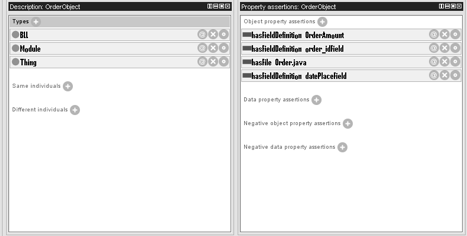
\includegraphics [scale=1.0] {OrderOWL}
  \caption{Представление класса Order в OWL. Визуализация Protege.} 
  \label{img:order-owl}  
\end{figure}


\begin{table} [htbp]
  \centering
  \parbox{17cm}{\caption{Описание свойств класса Order в OWL}\label{OrderPropertyDescription}}
%  \begin{center}
  \begin{tabular}{| p{5cm} | p{5cm} | p{7cm} |}
  \hline
  Свойство & Предикат & Описание \\
  \hline
    OrderAmount	& hasFieldDefinition & Поле: сумма заказа \\
  \hline
orderidField	& hasFieldDefinition & Поле: идентификатор заказа \\
  \hline
Order.java	& hasFile & Идентификатор имени файла для генерации \\
  \hline
datePlaceField	& hasFieldDefinition & Поле: время размещения заказа \\
  \hline
    \end{tabular}
%  \end{center}
\end{table}

\begin{table} [htbp]
  \centering
  \parbox{15cm}{\caption{Описание иерархии предикатов}\label{Predicates}}
%  \begin{center}
  \begin{tabular}{| p{5cm} | p{7cm} |}
  \hline
  
Предикат & Описание \\
  
    \hline
 hasFieldDefinition & Предикат, обозначающий свойство класса \\
  \hline
 hasMethodDefinition & Предикат, обозначающий функцию \\
  \hline
classDefinition & Обозначение класса \\
  \hline
database & Обозначение базы данных\\
  \hline
    \end{tabular}
%  \end{center}
\end{table}

\begin{figure} [h] 
  \center
  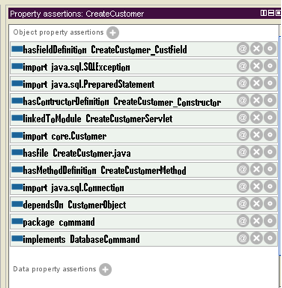
\includegraphics [scale=1.0] {CreateCustomer}
  \caption{Представление класса CreateCustiner в OWL. Визуализация Protege.} 
  \label{img:CreateCustomer}  
\end{figure}

\subsection{Основные компоненты модели}
Основными компонентами модели является:
\begin{enumerate}
	\item Request parser (Stanford parser)
	\item Генерация Action (Action Generator)
	\item Исполнение Action (Action Applier)
	\item Генерация приложения (Application Generator)
\end{enumerate} \par
\emph{Request parser} формализует запрос на естественном языке. \emph{Action Generator} генерирует Action объект из результатов работы парсера, основываясь на Деревьях принятия решений \cite{DCFOREST} и базе данных. Основной задачей данного модуля является генерация имени, действия и поля. Модуль \emph{Action Applier} ищет объект в модели по данным от Action Generator и производит действие, кроме того, используя предикат dependOn, он производит модификацию всех зависимых классов. В модели поддерживается два типа Action: RemoveFieldAction (удаление поля), AddFieldAction(добавление поля). После завершения работы производится генерация целевого приложения на языке Java при помощи OWL модели в модуле \emph{Application Generator}. На рисунке \ref{img:MentaUseCase} представлена диаграмма последовательности для основного рабочего потока. \par
\begin{figure} [h] 
  \center
  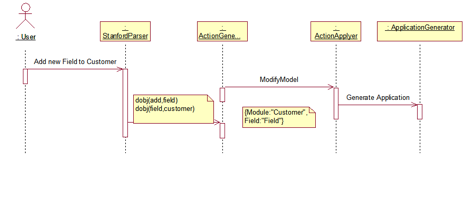
\includegraphics [scale=1.0] {MentaUseCase}
  \caption{Диаграмма последовательности для основного потока в модели Menta 0.1} 
  \label{img:MentaUseCase}  
\end{figure}

%===============================
\section{Модель Menta 0.3 с использованием Генетических алгоритмов} \label{chapt2}
После анализа ошибок была предпринята попытка сделать поиск решения более универсальным. В данной модели был добавлен модуль логики для оценки решения и модуль генетических алгоритмов для генерации решения. Генетические алгоритмы часто применяются в биологически инспирированных системах \cite{G1}, \cite{G3}. Кроме того, есть примеры использования и в система поддержки принятия решений, но эффективность таких систем не доказана \cite{G2}. В рамках данной модели были сформированы основные компоненты будущей модели:
\begin{itemize}
	\item Критерии Приемки (Acceptance Criteria)
	\item How-To для хранения решений проблем
	\item Формат данных OWL 
	\item Использование логических вычислений для проверки решения
\end{itemize} \par
Система содержала внутри себя модель приложения. При помощи генетического алгоритма модель строила из частей новую систему и проверяла ее при помощи логического движка NARS\cite{NARS} на соответствие входным критериям приемки, используя Fitness функцию для поколения \cite{GFITNESS}. 
\clearpage
\subsection{Основные компоненты модели}
Модель состоит из компонентов, представленных в Таблице \ref{ModulesMenta03}.

\begin{longtable}{|p{5cm}|p{10cm}|}
 \caption[Компонетны модели Menta 0.3]{Компонетны модели Menta 0.3}\label{ModulesMenta03} \\ 
 \hline
 
 \multicolumn{1}{|c|}{\textbf{Компонент}} & \multicolumn{1}{c|}{\textbf{Описание}}  \\ \hline 
\endfirsthead
\multicolumn{2}{c}%
{{\bfseries \tablename\ \thetable{} -- продолжение}} \\
\hline \multicolumn{1}{|c|}{\textbf{Компонент}} &
\multicolumn{1}{c|}{\textbf{Описание}}  \\ \hline 
\endhead

\hline \multicolumn{2}{|r|}{{Продолжение следует}} \\ \hline
\endfoot

\hline \hline
\endlastfoot
 MentaController & Веб-служба \cite{WebService}, который предоставляет интерфейс для общения с пользователем и остальными системами \\
  \hline
 SolutionGenerator & Модуль отвечает за генерацию решения. На вход он получает Acceptance Criteria. Основой является генетический алгоритм. Для него был выбран framework ecj \cite{ECJ} . Из всех возможных классов в базе знаний, отсеянных по классификатору составляются паросочетания. К каждому паросочетанию применяется логическое суждение на основе AcceptanceCriteria (за это отвечает модуль ReasonerAdapter). В итоге паросочетание получает оченку в виде пары Frequency, Confidence (частота, вероятность). 
Таким образом находится максимально лучше паросочетание. Если его показатель 1,1, то решение принимается, иначе отбрасывается (на данный момент установлен жесткий показатель).
SolutionGenerator включает в себя SolutionChecker, который включает в себя ReasonerAdapter.
 \\
  \hline
SolutionChecker & Проверка решения. Принимает на вход выбранные How-To, AcceptanceCriteria. Комбинирует их и передает ReasonerAdapter. \\
  \hline
ReasonerAdapter & Транслирует  How-To в термины NARS. NARS – non-axiomatic reasoning system \cite{NARS}. Система логических суждений, разработанная профессором Пеем Вонгом. Принцип ее действия~--- это всевозможная комбинация фактов. Каждый факт имеет свою частоту и вероятность. И по сочетанием получается композиция данных фактов.\\
  \hline
  Translator & Транслирует объекты базы знаний~--- знания~--- в отчеты. Отчеты бывают следующих типов:
  \begin{itemize}
  	\item Solution Report
  	\item UML Report
  	\item Patch
  \end{itemize} \par
В данной версии используется первый тип отчета. Этот отчет содержит описание решения, найденного системой на выбранном языке программирования.
\\
  \hline
  Applicator & Данный модуль применяет решение к модели приложения, содержащейся в базе знаний. Также данная модель включает FileApplicator, который генерирует решение в виде файлов на выбранном языке программирования. \\
  \hline
  KBServer & База знаний приложения. Используется сервер non-SQL БД HypergraphDB. \\
  \hline
%  \end{center}
\end{longtable}
\subsection{База знаний на основе графов}
При реализации KBServer был создан промежуточный слой DAO (Data Access Object), данный подход широко используется в проектировании программного обеспечения \cite{THREELAYERARCH}. Это позволяет максимально отделить реализацию KBServer от конкретного хранилища. 
\par \textbf{EntityManagerFactory} \par 
Данный класс представляет собой фабрику EntityManager, которая создает объекты класса EntityManager с одинаковыми настройками. Настройки могут быть переписаны.
\par \textbf{EntityManager} \par
Основной класс для загрузки, хранения объектов из базы данных.
\par \textbf{Configuration} \par
Класс хранит параметры настройки базы данных, такие как физическое положение БД, максимальное количество подключений.
\par \textbf{EntityTransaction}\par
Данный класс используется для управления транзакциями при доступе к объектам базы данных.

При выборе физического хранилища данных были исследованы несколько хранилищ OWL данных: OWLIM, SESAME и HG. Результаты их сравнения приведены в таблице \ref{DatabaseEngineComparison}.
\begin{longtable}{|p{5cm}|p{3cm}|p{3cm}|p{3cm}|}
 \caption[Сравнение скорости доступа к данным баз знаний]{Сравнение скорости доступа к данным баз знаний}\label{DatabaseEngineComparison} \\ 
 \hline
 
 \multicolumn{1}{|c|}{\textbf{}} & \multicolumn{1}{c|}{\textbf{Sesame}} & \multicolumn{1}{c|}{\textbf{OWLIM}} & \multicolumn{1}{c|}{\textbf{HG}} \\ \hline 
\endfirsthead
\multicolumn{2}{c}%
{{\bfseries \tablename\ \thetable{} -- продолжение}} \\
\hline \multicolumn{1}{|c|}{\textbf{}} & \multicolumn{1}{c|}{\textbf{Sesame}} & \multicolumn{1}{c|}{\textbf{OWLIM}} & \multicolumn{1}{c|}{\textbf{HG}} \\ \hline 
\endhead

\hline \multicolumn{2}{|r|}{{Продолжение следует}} \\ \hline
\endfoot

\hline \hline
\endlastfoot
 nanoseconds & select 10 & select 10 & select 10 \\
  \hline
 with compilation & 26253058 & 3012115 & 6813994 \\
  \hline
  not cached & 30545223 & 1122210 & 9045563 \\
  \hline
  cached & 24258390 & 962972 & 985041 \\
  \hline 
%  \end{center}
\end{longtable}

Несмотря на то, что OWLIM дает лучшее результаты, был выбран HGDB, так как он предоставляет более широкие возможности доступа к данным, такие как поддержка алгоритмов работы с графами.

%========================================
%========================================

\section{Модель TU 1.0, основанная на модели мышления Марвина Мински}
Следующим этапом стала модель, построенная с применением теории Марвина Мински, которая содержала в себе основные концепции предыдущих моделей и показала свою состоятельность на контрольных примерах.
\begin{itemize}
	\item Acceptance Criteria
	\item Обучение
	\item Поиск и применение решения 
	\item Отсутсвие обработки естественного языка
\end{itemize} \par
Данная модель является более универсальной и представляет собой верхнеуровневую архитектуру обработки запроса (мышления), где компонентами являются лучшие части предыдущих систем.
\subsection{Особенности модели мышления}
В 2006 году Марвин Мински опубликовал свою книгу "The emotion machine" \cite{EmotionMachine}, в которой предложил свой взгляд на систему мышления и памяти человека. В основу теории легла парадигма триплета Критик-Селектор-Путь мышления, k-line для сопоставления знаний. На рисунке \ref{img:csw} представлена схематичное изображение Критика-Селектора-Пути мышления. \par
\begin{figure} [h] 
  \center
  \includegraphics [scale=1.0] {CSW}
  \caption{Критик-Селектор-Путь мышления} 
  \label{img:csw}  
\end{figure}

\textbf{Критик} представляет собой определенный триггер: внешние обстоятельства, события или иное воздействие. Например, включился свет и зрачки сузились, обожглись и одернули руку. Критик активируется только когда для этого достаточно обстоятельств. Одновременно могут активироваться несколько критиков. Например, человек решает сложную задачу. Идет активация множество критиков: считать, технические детали, кроме того параллельно может активироваться критик переработки, сообщающей о необходимости отдыха.\par
\textbf{Селектор} занимается выбором определенных ресурсов, которыми также являются Пути мышления. \par
\textbf{Путь мышления} это способ решения проблемы. Путь мышления также может активировать следующий критик. \par

На рисунке \ref{img:csw_ex} представлена расширенная модель работы триплета Критик-Селектор-Путь мышления. Критик активирует селектор, который активирует путь мышления (синий круг). Путь мышления в свою очередь может активировать критик или же совершить определенные действия. Например, зажегся зеленый свет светофора, значит можно переходить дорогу. \par
Если активировалось много критиков, значит проблему нужно уточнить, так как степень неопределенности слишком высока. Если проблема очень похожа, то можно судить по аналогии.
\begin{figure} [h] 
  \center
  \includegraphics [scale=1.0] {CSW_EX}
  \caption{Критик-Селектор-Путь мышления в разрезе ресурсов} 
  \label{img:csw_ex}  
\end{figure}

\clearpage
\subsection{Основные компоненты модели}
\subsubsection{Уровни мышления}
Концепция уровней мышления представляет собой модель степени ментальной активности человека. Никто из людей не может похвастаться скоростью гепарда, гибкости кошки, силой медведя. Но наш вид все это компенсирует возможностью изобретения образов мышления. Например, чтобы быть быстрыми мы изобрели самолеты, машины. Чтобы быть сильными, мы изобрели оружие. Что же делает это возможным? Безусловно результатом всего является взаимодействие человека с окружающим миром. Именно данное взаимодействие заставляет людей изобретать что-то новое, создавать шедевры литературы и летать в космос. Но как же мы всего этого добиваемся, начиная от инстинктивного одергивания руки до создания Теории всего \cite{Hawking}. Далее мы рассмотрим концепцию уровней мышления. \par
\begin{enumerate}
	\item Инстинктивный уровень
	\item Уровень обученных реакций
	\item Уровень рассуждений
	\item Рефлексивный уровень
	\item Саморефлексивный уровень
	\item Самосознательный уровень
\end{enumerate} \par

В Таблице \ref{ThinkingLevelDescription} представлено описание уровней мышления.
\begin{table} [htbp]
  \centering
  \parbox{15cm}{\caption{Описание уровней мышления Марвина Мински}\label{ThinkingLevelDescription}}
%  \begin{center}
  \begin{tabular}{| p{5cm} | p{11cm} |}
 
  \hline
\textbf{Уровень} & \textbf{Описание} \\
  \hline
 
Инстинктивный уровень	& На данном уровне происходят инстинктивные реакции (врожденные). Например, боязнь обжечься. Не прыгать под машину. Общую формулу для этого уровня можно выразить как "Если ..., то сделать так". \\
  \hline

Уровень обученных реакций  & На данном уровне происходит мышление обученных реакций, то есть тех реакций, которыми человек обучается в течение жизни. Например, переходить дорогу на зеленых свет. Общую формулу для этого уровня можно выразить как "Если ..., то сделать так". \\
  \hline

Уровень рассуждений & На данном уровне происходит мышление с использованием рассуждений. Если я сделаю так, то будет ... Например, если перебежать дорогу на зеленый свет, то можно успеть вовремя. Здесь сравниваются последствия нескольких решений и выбирается оптимальное. Общую формулу для этого уровня можно выразить как "Если ..., то сделать так, тогда будет так". \\
  \hline

Рефлексивный уровень  & На данном уровне происходит рассуждение с учетом анализа прошлых событий. Например, прошлый раз я побежал на моргающий зеленый и чуть не попал под машину. \\

  \hline
  Саморефлексивный уровень & На данном уровне происходит оценка себя. Строится определенная модель с помощью которой идет оценка своих поступков. Например, мое решение не пойти на это собрание было неверным, так как я упустил столько возможностей, я был легкомысленный. \\
  \hline
  Самосознательный уровень & На данный момент характерен только для человека. На данном уровне идет оценка поступков человека с точки зрения высших идеалов и внешних оценок. Например, а что подумают мои друзья? А как бы поступил мой герой? \\
  \hline
  
  \end{tabular}
%  \end{center}
\end{table}

Деление на данные уровне носит условный характер. Например уровень 5 и 6 можно объединить. Но по словам Марвина Мински принцип бритвы Оккама, который успешно применяется в физике, не должен также легко и однозначно применяться в психологии и теории мышления. \par
На рисунке \ref{img:thinkinglevels} представлено схематичное изображение уровней мышления. 1-3 уровни составляют личность человека. 2-5 представляют ЭГО человека (Человеческое Я) - осознание человека в общении с окружающими. 3-6 представляют собой сверх ЭГО человека (сверх Я) - его моральные установки.
\begin{figure} [h] 
  \center
  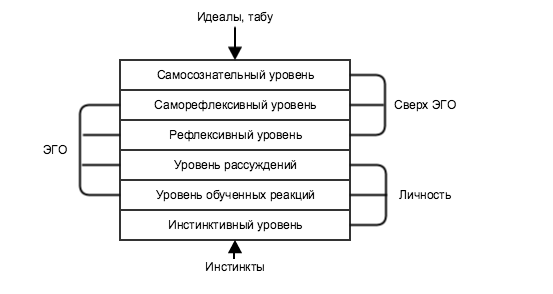
\includegraphics [scale=1.0] {thinkinglevels}
  \caption{Иллюстрация концепции Уровней мышления} 
  \label{img:thinkinglevels}  
\end{figure}
\clearpage
\subsubsection{K-line}
Концепция K-line была первый раз упомянута Марвином Мински в 1987 году в журнале Cognitive Science. В книге "The Society of Mind" \cite{SocietyOfMind} Марвин Мински раскрывает концепцию K-line. Полностью концепция описана позже в книге "The Emotion Machine" \cite{EmotionMachine}. 
K-line представляет собой связь между двумя событиями, объединяющими их в знание. Например, объединение Пути мышления, найденного решения и активированной проблемы. Данная линия объединяет то как мы думали, решение.
\begin{figure} [h] 
  \center
  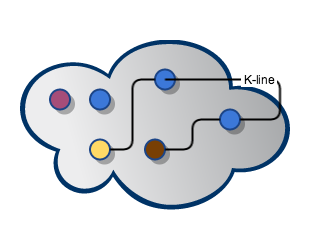
\includegraphics [scale=1.0] {k_line}
  \caption{Иллюстрация концепции K-line} 
  \label{img:k_line}  
\end{figure}
На Рисунке \ref{img:k_line} показана K-line, которая объединяет пути мышления, решение и другие Критики. Данная концепция позволяет "запоминать" удачные решения. 
\clearpage

\section{Выводы}
Модель Menta 0.1 имеет следующие недостатки
\begin{enumerate}
	\item Отсутствие устойчивости к ошибкам входной информации: грамматическим и содержательным. Например, входной файл не имел отношения к программной системе, модель которой была в базе знаний в формате OWL
	\item Система поиска решения работала только в рамках модели одной программы
	\item Отсутствовала функция обучения 
\end{enumerate}\par
В данный момент существует новый подход, который использует леса деревьев принятия решений \cite{DCFOREST}, он в рамках данной модели не рассматривался.
Модель Menta 0.3 имеет следующие недостатки:
\begin{itemize}
	\item Отсутсвие обучения
	\item Отсутсвие обработки естественного языка
	\item HyperGraphDB оказалась непригодный для промышленного использования
	\item NARS в виду своих особенностей оказался непригодным для промышленного применения на значительном объеме фактов (>20). Так как содержал в себе комбинаторный взрыв. Например при 10 фактов количество сочетаний будет равно 45 на первом уровне, далее будут сравнивать результаты этих сочетаний.  
	\item Апробации оказалось, что критерии приемки практически описывают необходимое решение, что являлось недопустимым. Данный подход был описан в статье \cite{SECR}.
\end{itemize}\par
Для программной экспертной системы очень важно обладать способностью мыслить и рассуждать. Например, очень важно  для системы уметь действовать по аналогии. Так как множество запросов типичны и отличаются лишь параметрами. Например, пожалуйста, установить Office, Antivirus и т.д. \par
Также для экспертной системы важно уметь абстрагировать специализированные рецепты решения. К примеру, система научилась решать инцидент "Please install Firefox". Абcтрагировав данный инцидент до степени "Please install browser" система сможет теми же способами попробовать решить новый инцидент.\par
После рассмотрения нескольких моделей была выбрана модель мышления Марвина Мински, так как данная модель наиболее точно ложится на целевую область решения инцидентов в области IT. На основе подхода Мински была построена модель системы, которая поддерживает основные функции: обучение, понимание инцидента, поиск решения, применение решения. Более подробно с результатами апробации моделей можно ознакомиться на сайте http://tu-project.com

\clearpage

